% XeLaTeX

\documentclass{article}
\usepackage{ctex}
\usepackage{xypic}
\usepackage{amsfonts,amssymb}
\usepackage{multirow}
\usepackage{geometry}
\usepackage{graphicx}
\usepackage{listings}
\usepackage{lipsum}
\usepackage{courier}
\usepackage{fancyvrb}
\usepackage{etoolbox}


\linespread{1.2}
\geometry{left=3cm,right=2.5cm,top=2.5cm,bottom=2.5cm}

\makeatletter
\patchcmd{\FV@SetupFont}
  {\FV@BaseLineStretch}
  {\fontencoding{T1}\FV@BaseLineStretch}
  {}{}
\makeatother

\lstset{basicstyle=\small\fontencoding{T1}\ttfamily,breaklines=true}
\lstset{numbers=left,frame=shadowbox,tabsize=4}
%\lstset{extendedchars=false}
\begin{document}

\title{Project 3 实验报告}
\author {姓名:王凯祺 \text{ } 学号:16337233 \text{ } 班级:教务3班}
\maketitle

\section{需求分析}

实现一个多项式计算器,支持以下功能:

1. 输入多项式并保存到内存。

2. 多项式相加。

3. 多项式相减。

4. 多项式与常数的乘法运算。

5. 求多项式代入某点的值。

6. 显示内存中的多项式。

7. 多项式与多项式相乘。

8. 判断两个多项式是否相等。

9. 对一个多项式求导。

要求:

1. 支持将计算结果保存为变量。

2. 输入的多项式可以为之前保存过的变量。

\section{实现思路}

\begin{figure}[!hbp]
	\centering
	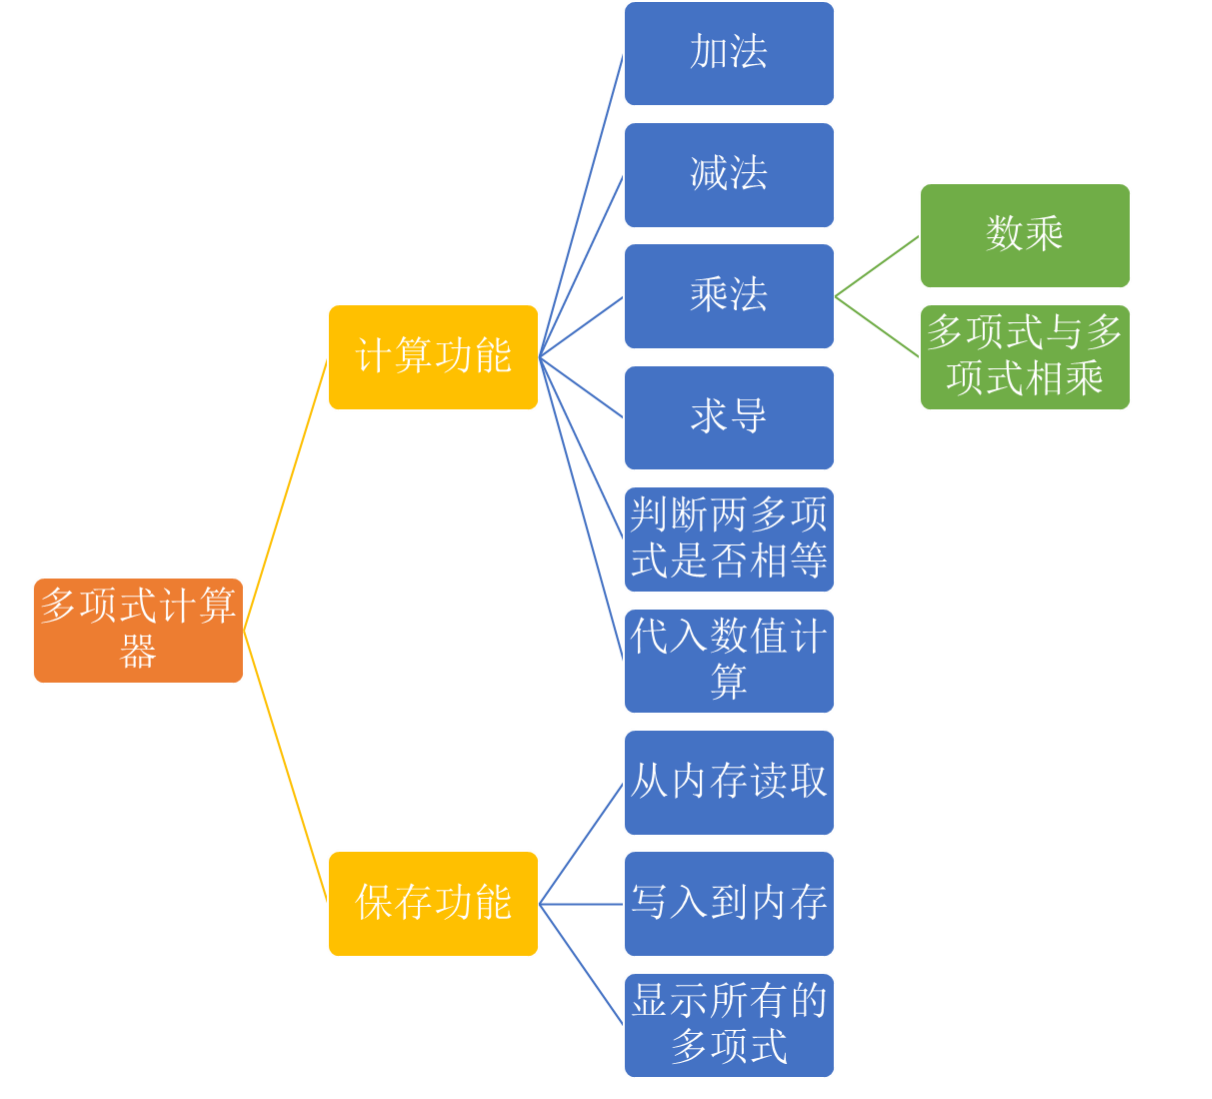
\includegraphics[scale=0.4]{s1.png}
\end{figure}

\subsection{计算功能}

创建一个多项式类,用 vector 容器存储从低次到高次的项。

加法:记相加的两个多项式为 $a, b$ ,其次数为 $d_a, d_b$ ,则 $a + b$ 的次数不超过 $max(d_a, d_b)$ ,对位相加后化简即可。

减法:记减法的两个多项式为 $a, b$ ,其次数为 $d_a, d_b$ ,则 $a + b$ 的次数不超过 $max(d_a, d_b)$ ,对位相减后化简即可。

数乘:记该多项式为 $a$ ,其次数为 $d_a$ ,则 $a$ 的次数不超过 $d_a$ (不一定就是 $d_a$ ,因为与其相乘的常数可能为 $0$ ),对位相乘后化简即可。

多项式乘法:记相乘的两个多项式为 $a, b$ ,其次数为 $d_a, d_b$ ,则 $a + b$ 的次数不超过 $d_a + d_b)$ ,用 $O(n^2)$ 求一个卷积后化简即可。

求导:记该多项式为 $a$ ,其次数为 $d_a$ ,则 $a$ 的次数不超过 $max(d_a - 1, 0)$ (不一定就是 $d_a - 1$ ,因为与 $d_a$ 可能为 $0$),简单求个导即可。

判断多项式相等:先判次数,再对每个项分别判一下即可。

\subsection{保存功能}

用个 map 映射一下,把 string 映射成多项式的类即可。

从 map 中读取:先用 map::find 找一下是否有这样的变量,若有就返回该多项式;否则新建一个多项式。

写入到 map :map[name] = polynomial。

显示所有的多项式:遍历整个 map。

\section{数据设计}

一个 vector 就能表示一个多项式了呀 :)

\begin{lstlisting}[language=C++]
class poly {
    vector<int> c;
};
\end{lstlisting}

\section{类设计和函数设计}

函数设计也十分简单啊,对于每个功能重载一个运算符或者写一个函数即可。

\begin{lstlisting}[language=C++]
class poly {
public:
    poly();
    friend istream& operator >> (istream &in, poly &a);
    friend ostream& operator << (ostream &out, const poly &a);
    poly operator + (const poly &rhs);
    poly operator - (const poly &rhs);
    poly operator * (const int rhs);
    poly operator * (const poly &rhs);
    bool operator == (const poly &rhs);
    void optim(); // 化简多项式
    int solve(int x) const; // 代入 x 求值
    poly derivative(); // 多项式求导
    int valid(); // 是否为合法的多项式
private:
    vector<int> c;
};
\end{lstlisting}

\section{输入与输出}

\subsection{输入}

先输入一个字符串进来,从头扫到尾。

容易找到所有的左括号,从左括号开始遍历到下一个右括号,经过恰好一个逗号和两个数,将这两个数加到对应的项即可。

\subsection{输出}

从高位往低位输出,遇到 0 就跳过,遇到次数为 1 或 -1 、系数为 1 或 -1 的特判一下即可。

\end{document}
















